\chapter{Evaluation}

I evaluated the following cool thing...

The pair encoding scheme still does significant work reduction after the loop finder runs, showing there is more general 
redundancy 

\section{Methodology}

Talk about how results were acquired

\section{Algorithmic and data-driven optimisations}

\begin{figure}[htbp]
  \centering
  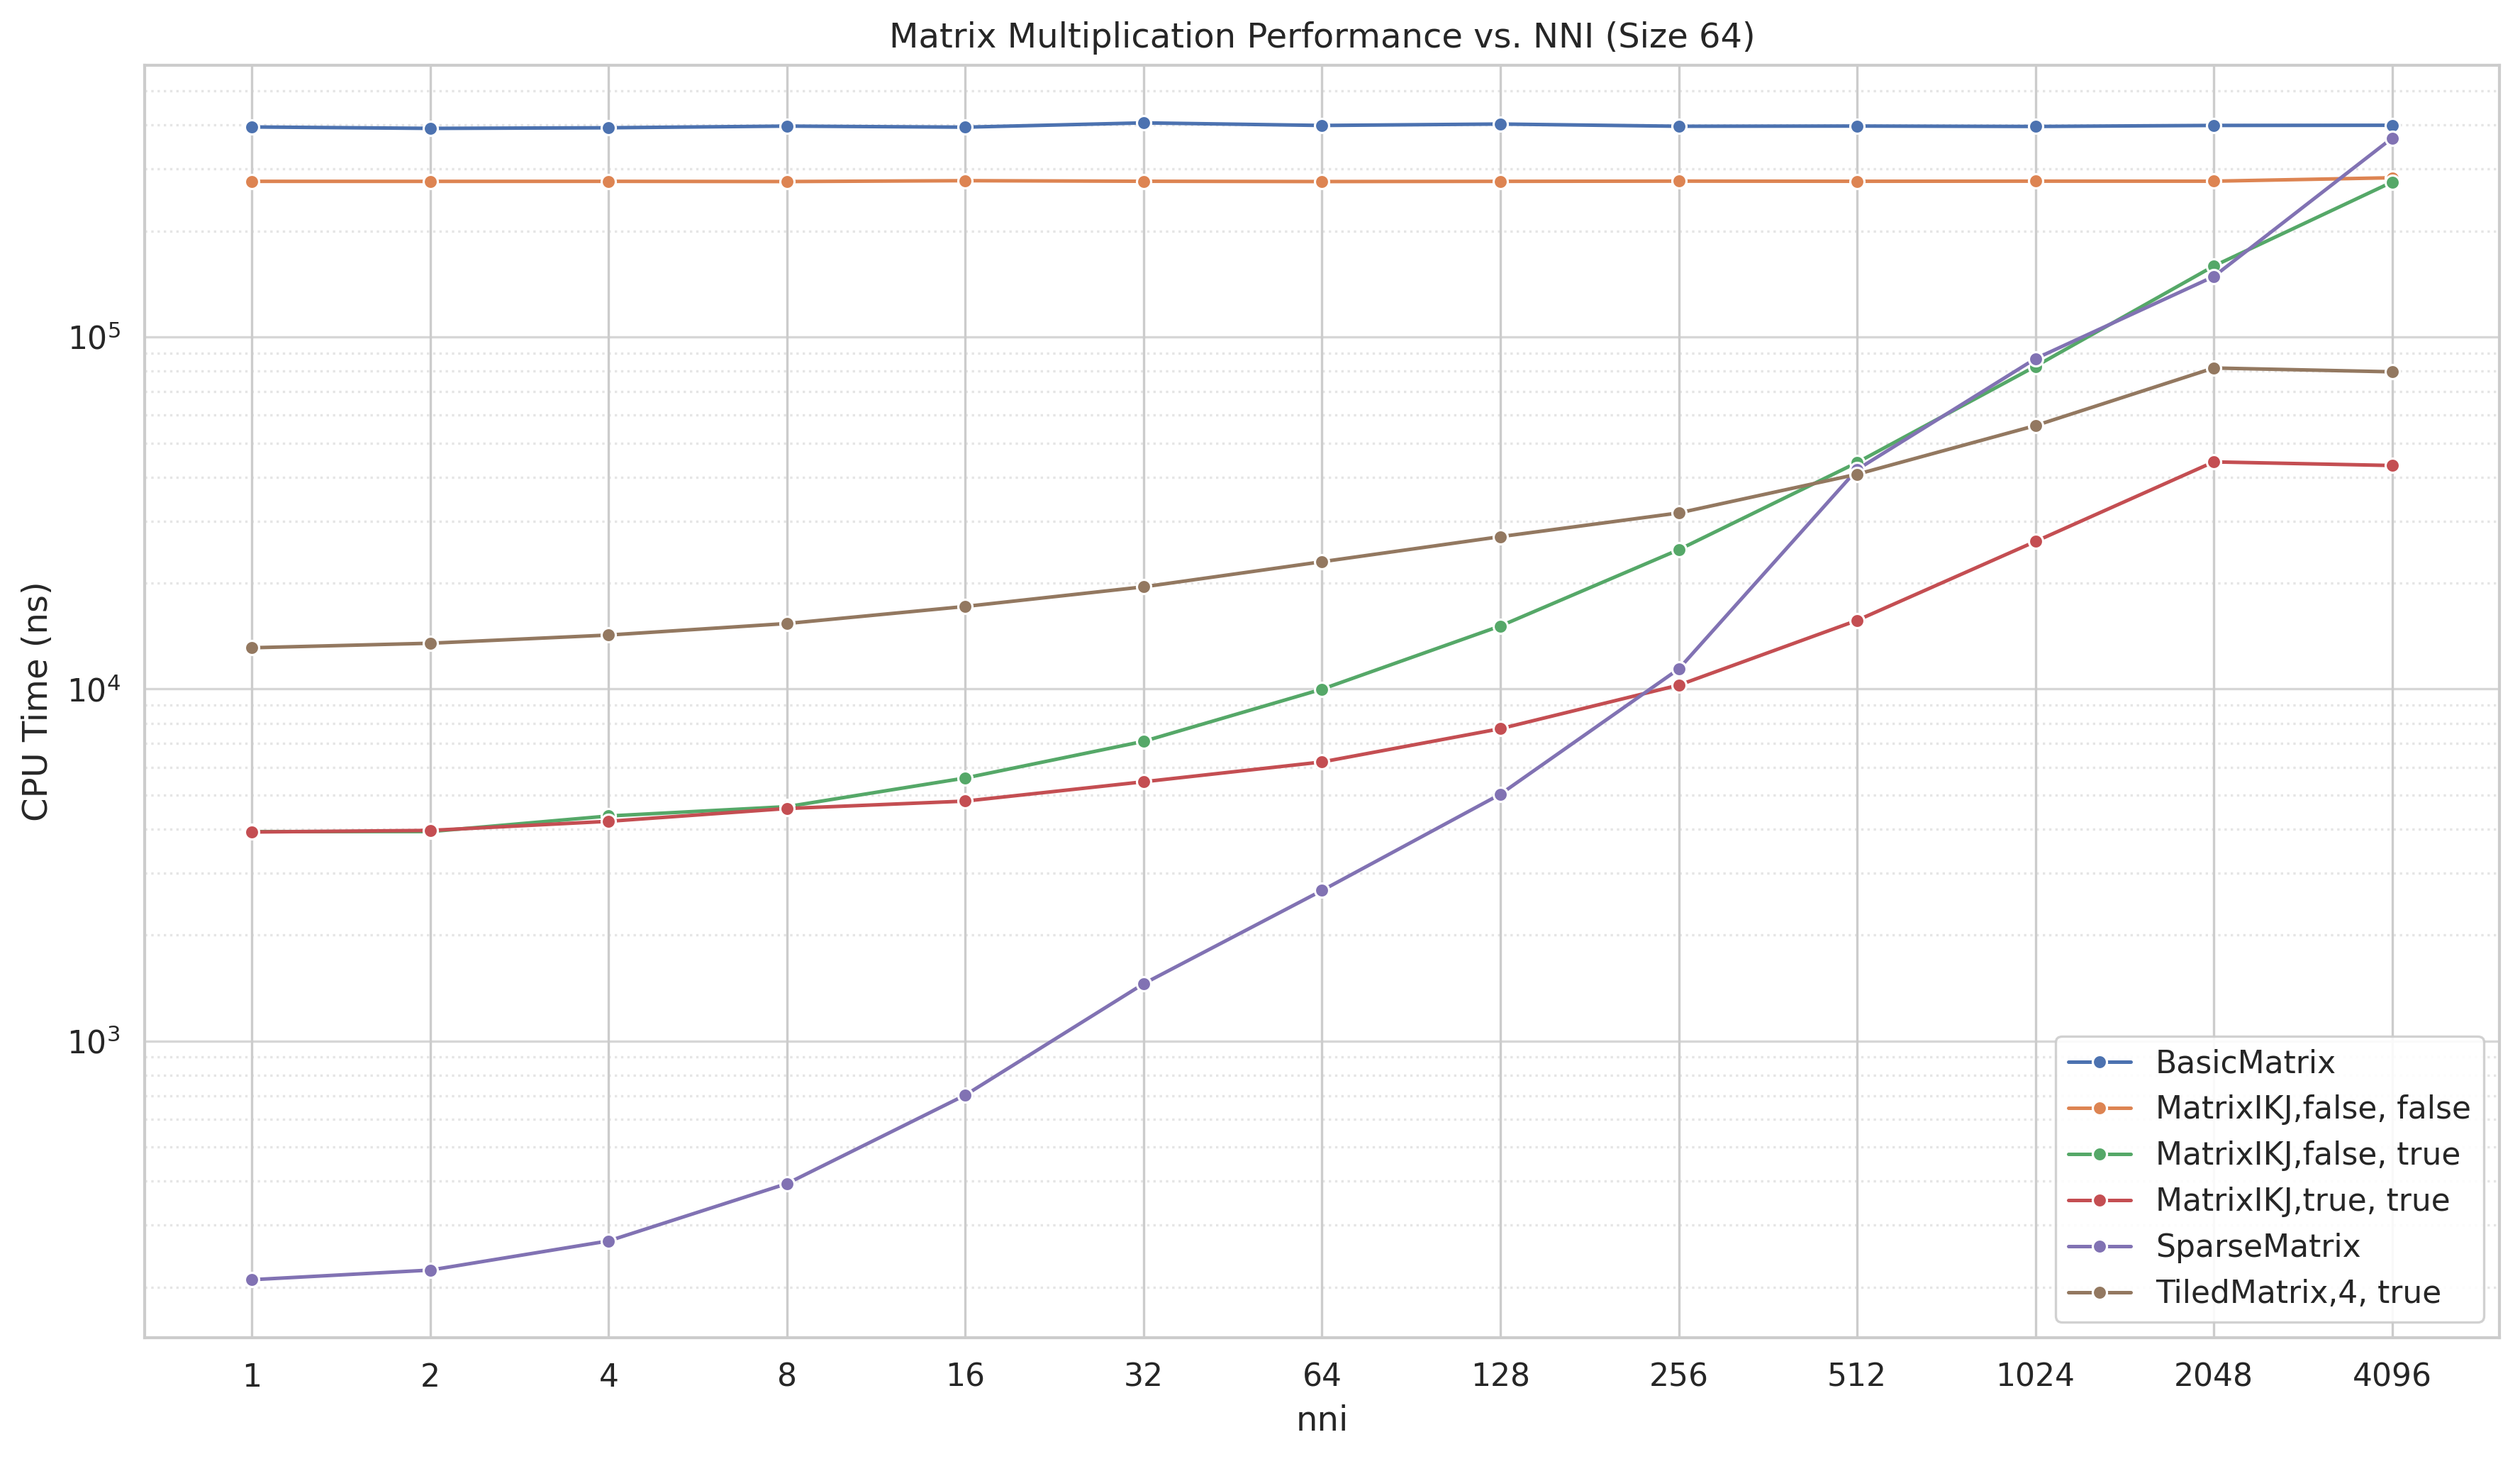
\includegraphics[width=0.5\textwidth]{graphs/matrix_nni_performance.png}
  \caption{Comparing runtime of matrix multiplication approaches, for matrices of varying sparsity.}
  \label{eval:fig:matrix-perf}
\end{figure}

Parameter sweet spots for encoding - minimise parameters 

\begin{figure}[htbp]
  \centering
  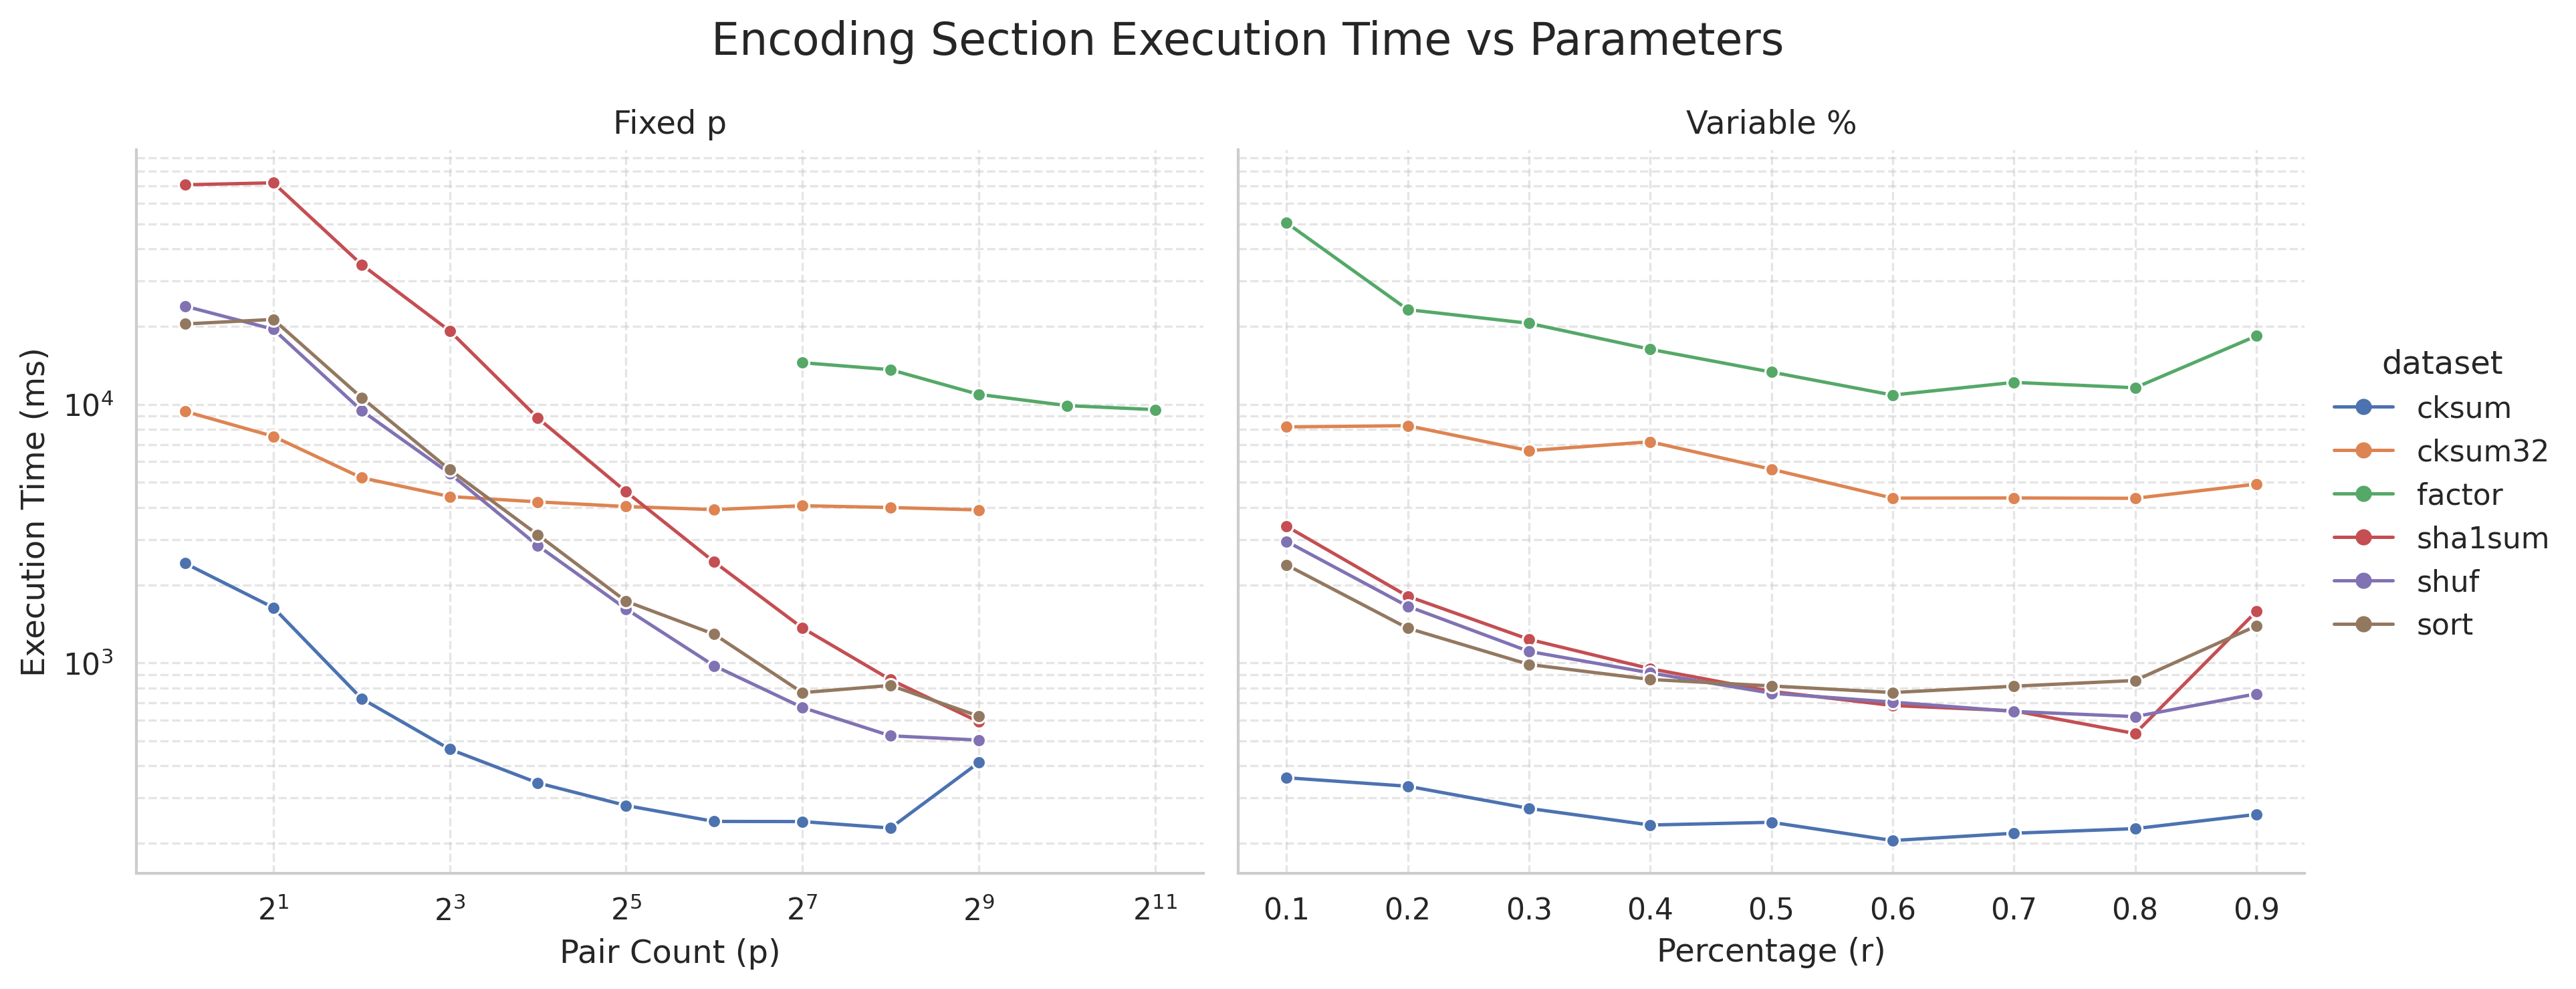
\includegraphics[width=0.8\textwidth]{graphs/encoder_time.png}
  \caption{Comparing runtime of program on different datasets, for different encoder parameters, excluding block 
  preprocessing and loop finding.}
  \label{eval:fig:encoder-perf}
\end{figure}

\begin{figure}[htbp]
  \centering
  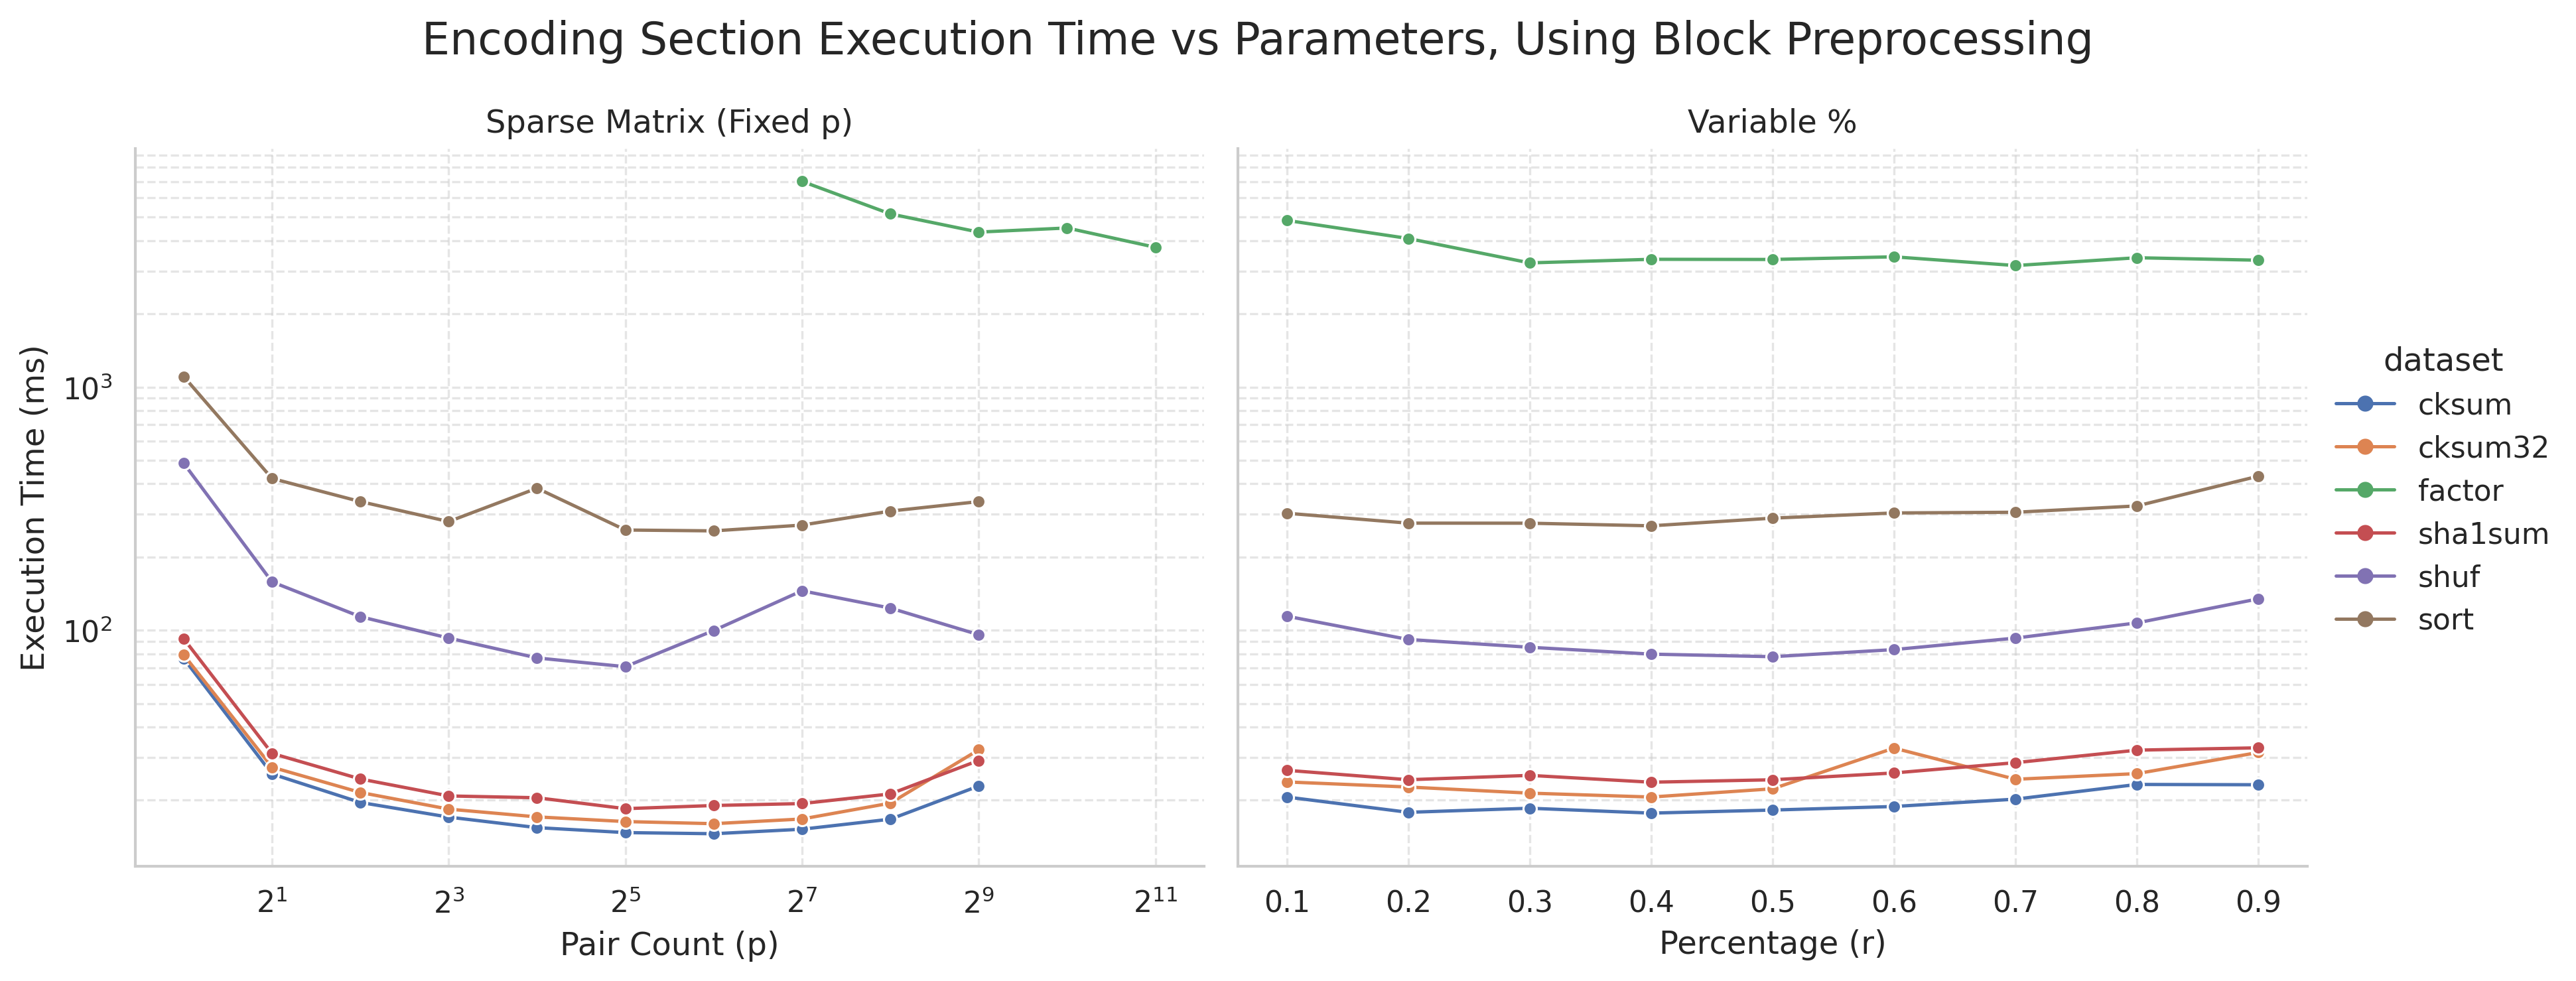
\includegraphics[width=0.8\textwidth]{graphs/encoder_time_block.png}
  \caption{Comparing runtime of program on different datasets, for different encoder parameters, including block 
  preprocessing.}
  \label{eval:fig:encoder-block-perf}
\end{figure}

\begin{figure}[htbp]
  \centering
  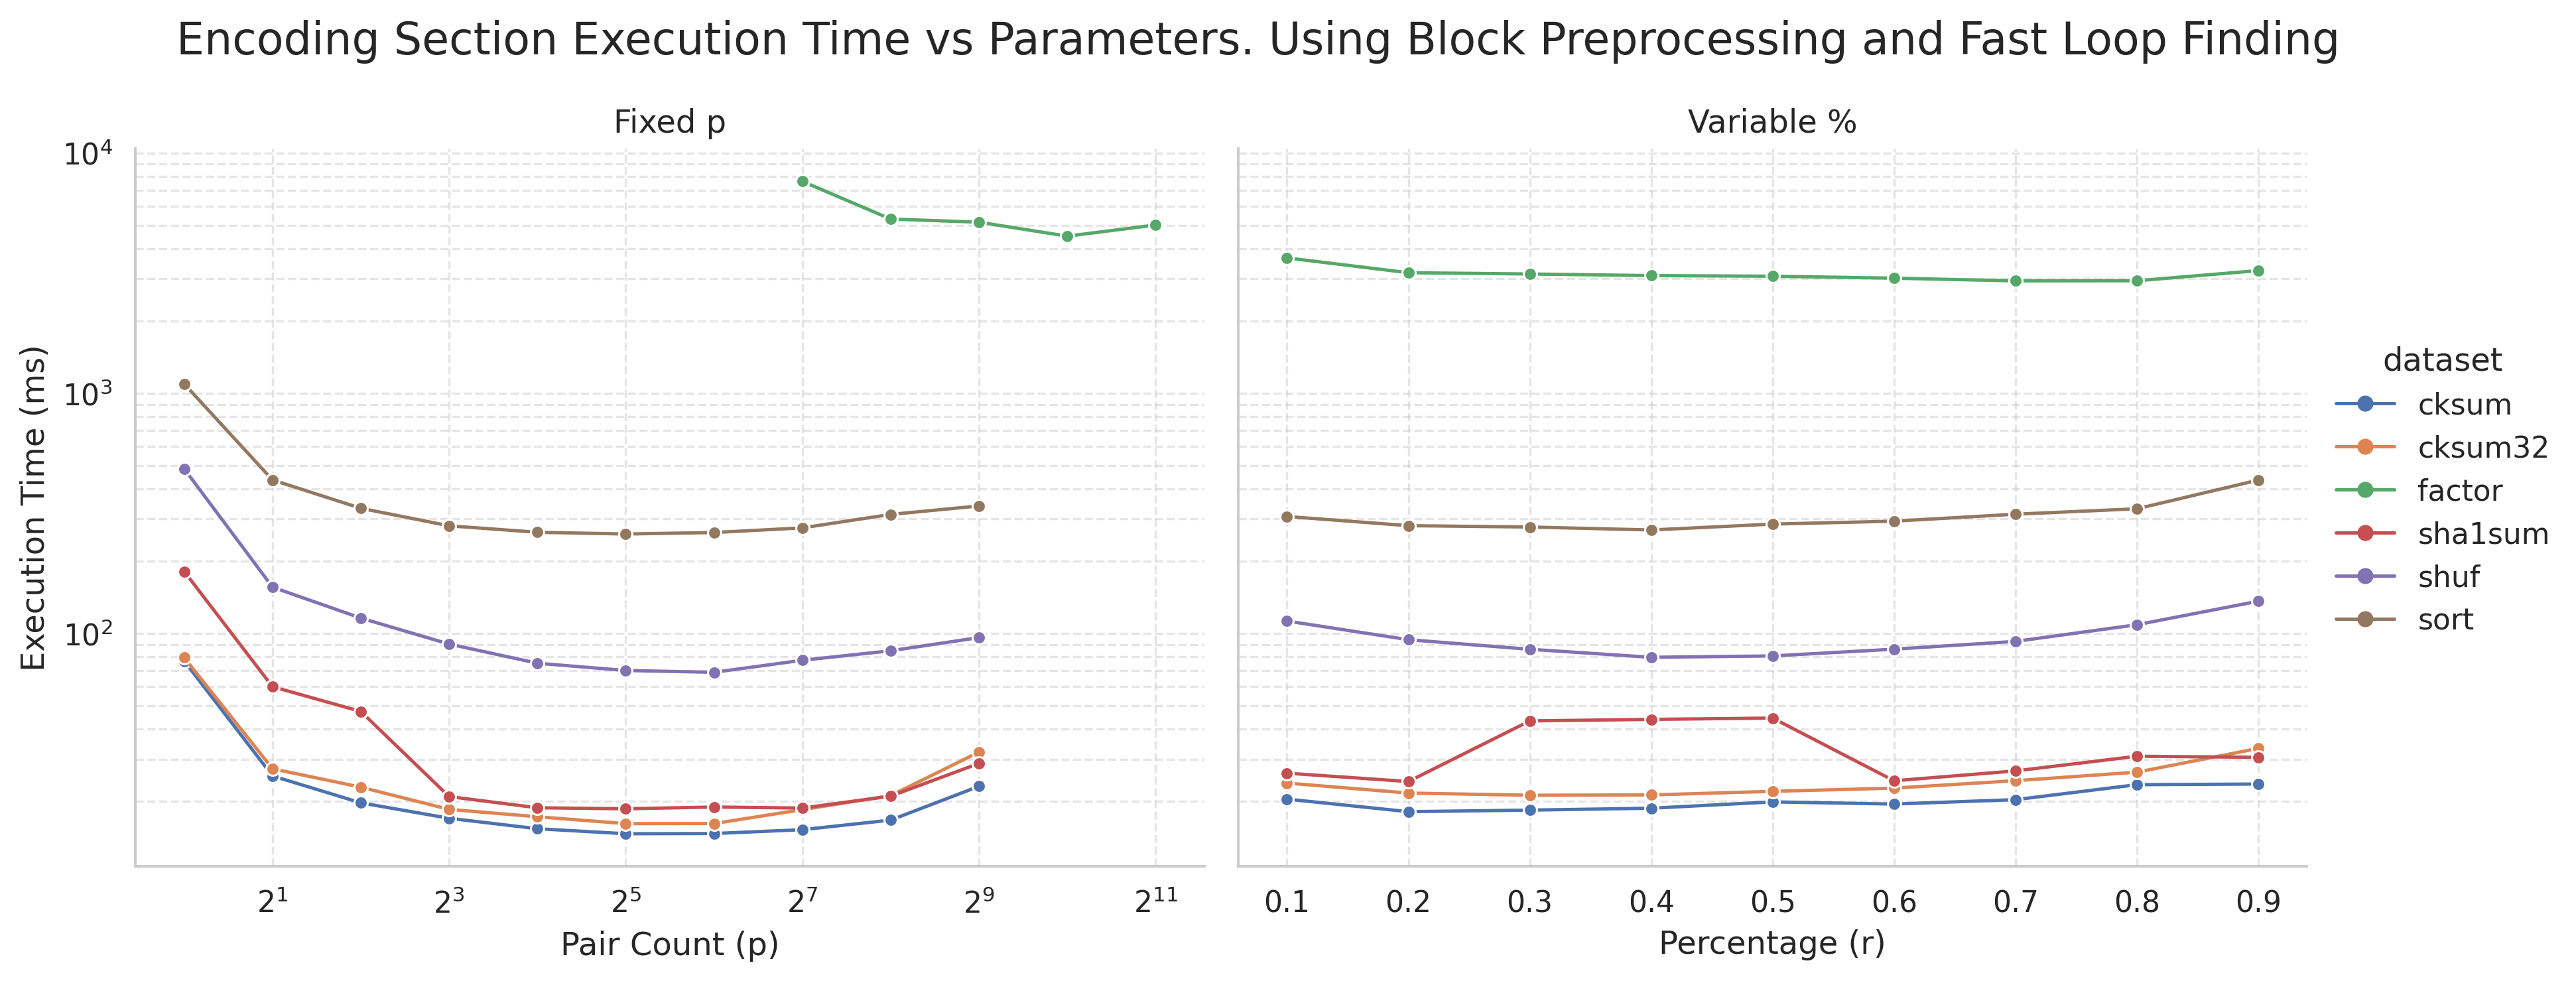
\includegraphics[width=0.8\textwidth]{graphs/encoder_time_loop.png}
  \caption{Comparing runtime of program on different datasets, for different encoder parameters, including block 
  preprocessing and loop finding.}
  \label{eval:fig:encoder-block-loop-perf}
\end{figure}

Compression ratio for encoders.

\begin{figure}[htbp]
  \centering
  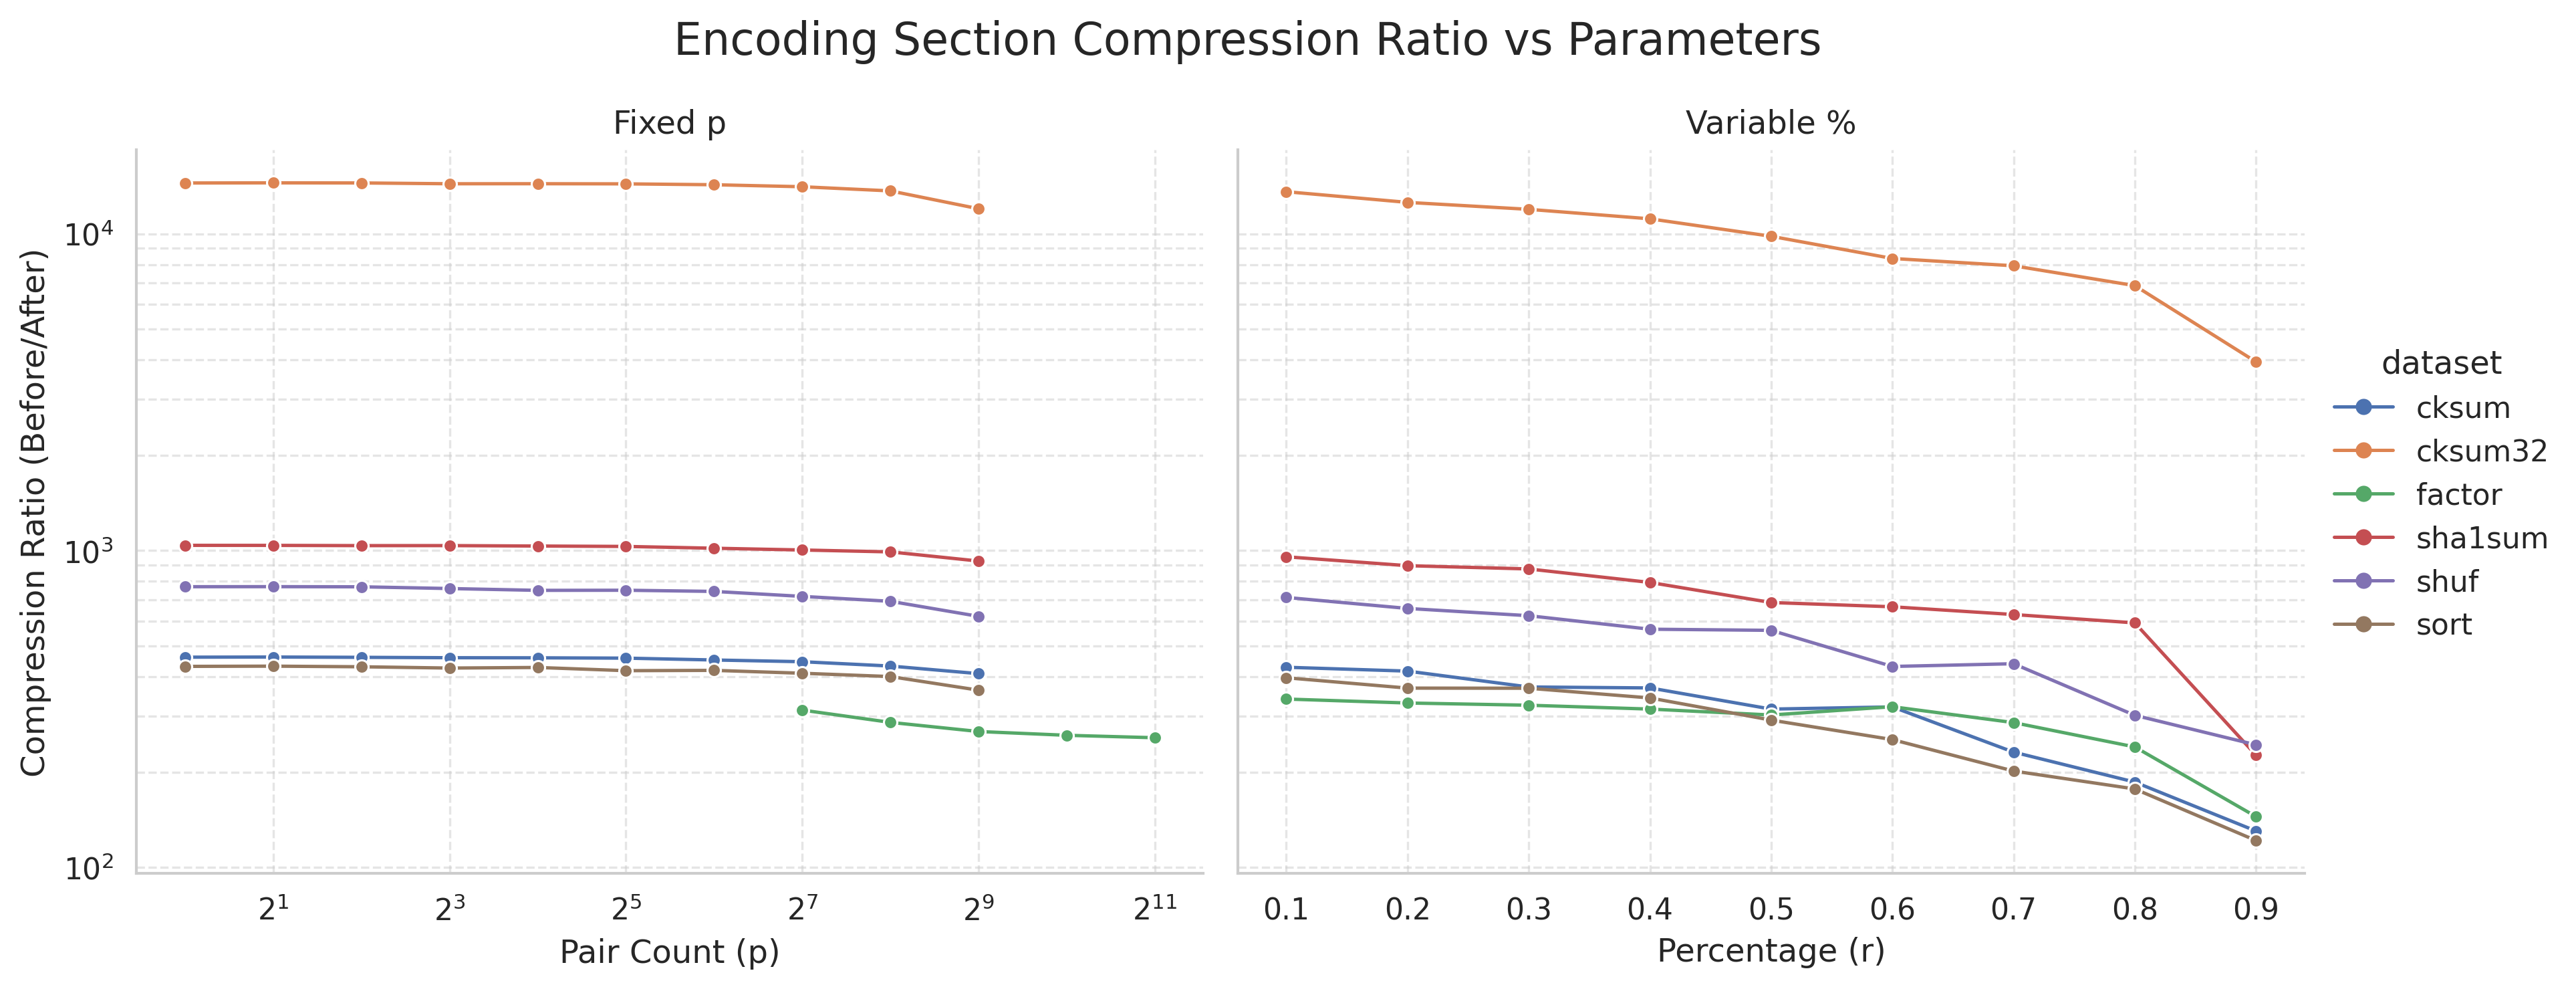
\includegraphics[width=0.8\textwidth]{graphs/encoder_compression.png}
  \caption{Comparing compression ratio of encoder on different datasets, for different encoder parameters, excluding block 
  preprocessing and loop finding.}
  \label{eval:fig:encoder-comp}
\end{figure}

\begin{figure}[htbp]
  \centering
  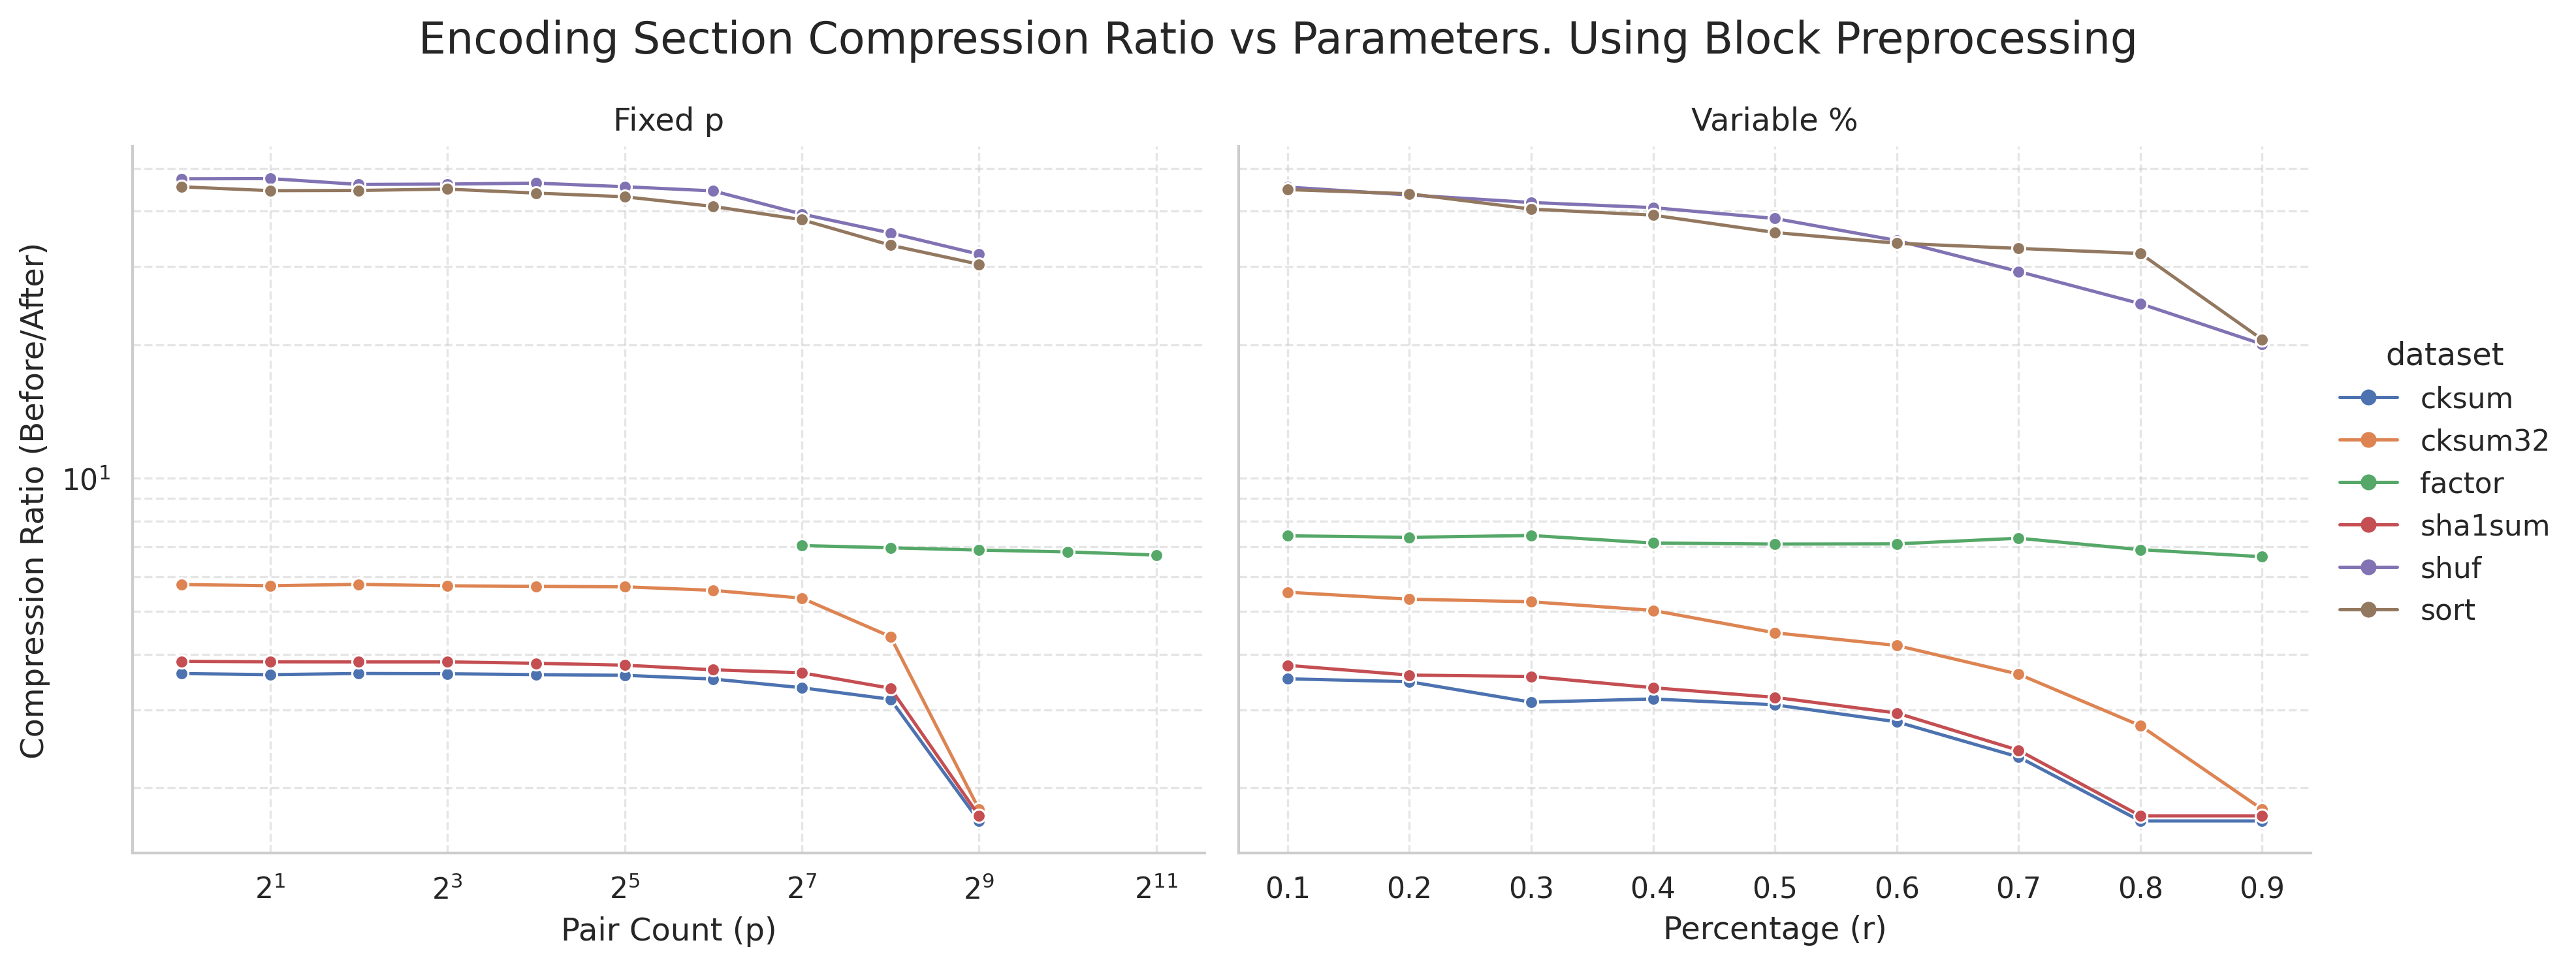
\includegraphics[width=0.8\textwidth]{graphs/encoder_compression_block.png}
  \caption{Comparing runtime of program on different datasets, for different encoder parameters, including block 
  preprocessing.}
  \label{eval:fig:encoder-block-comp}
\end{figure}

\begin{figure}[htbp]
  \centering
  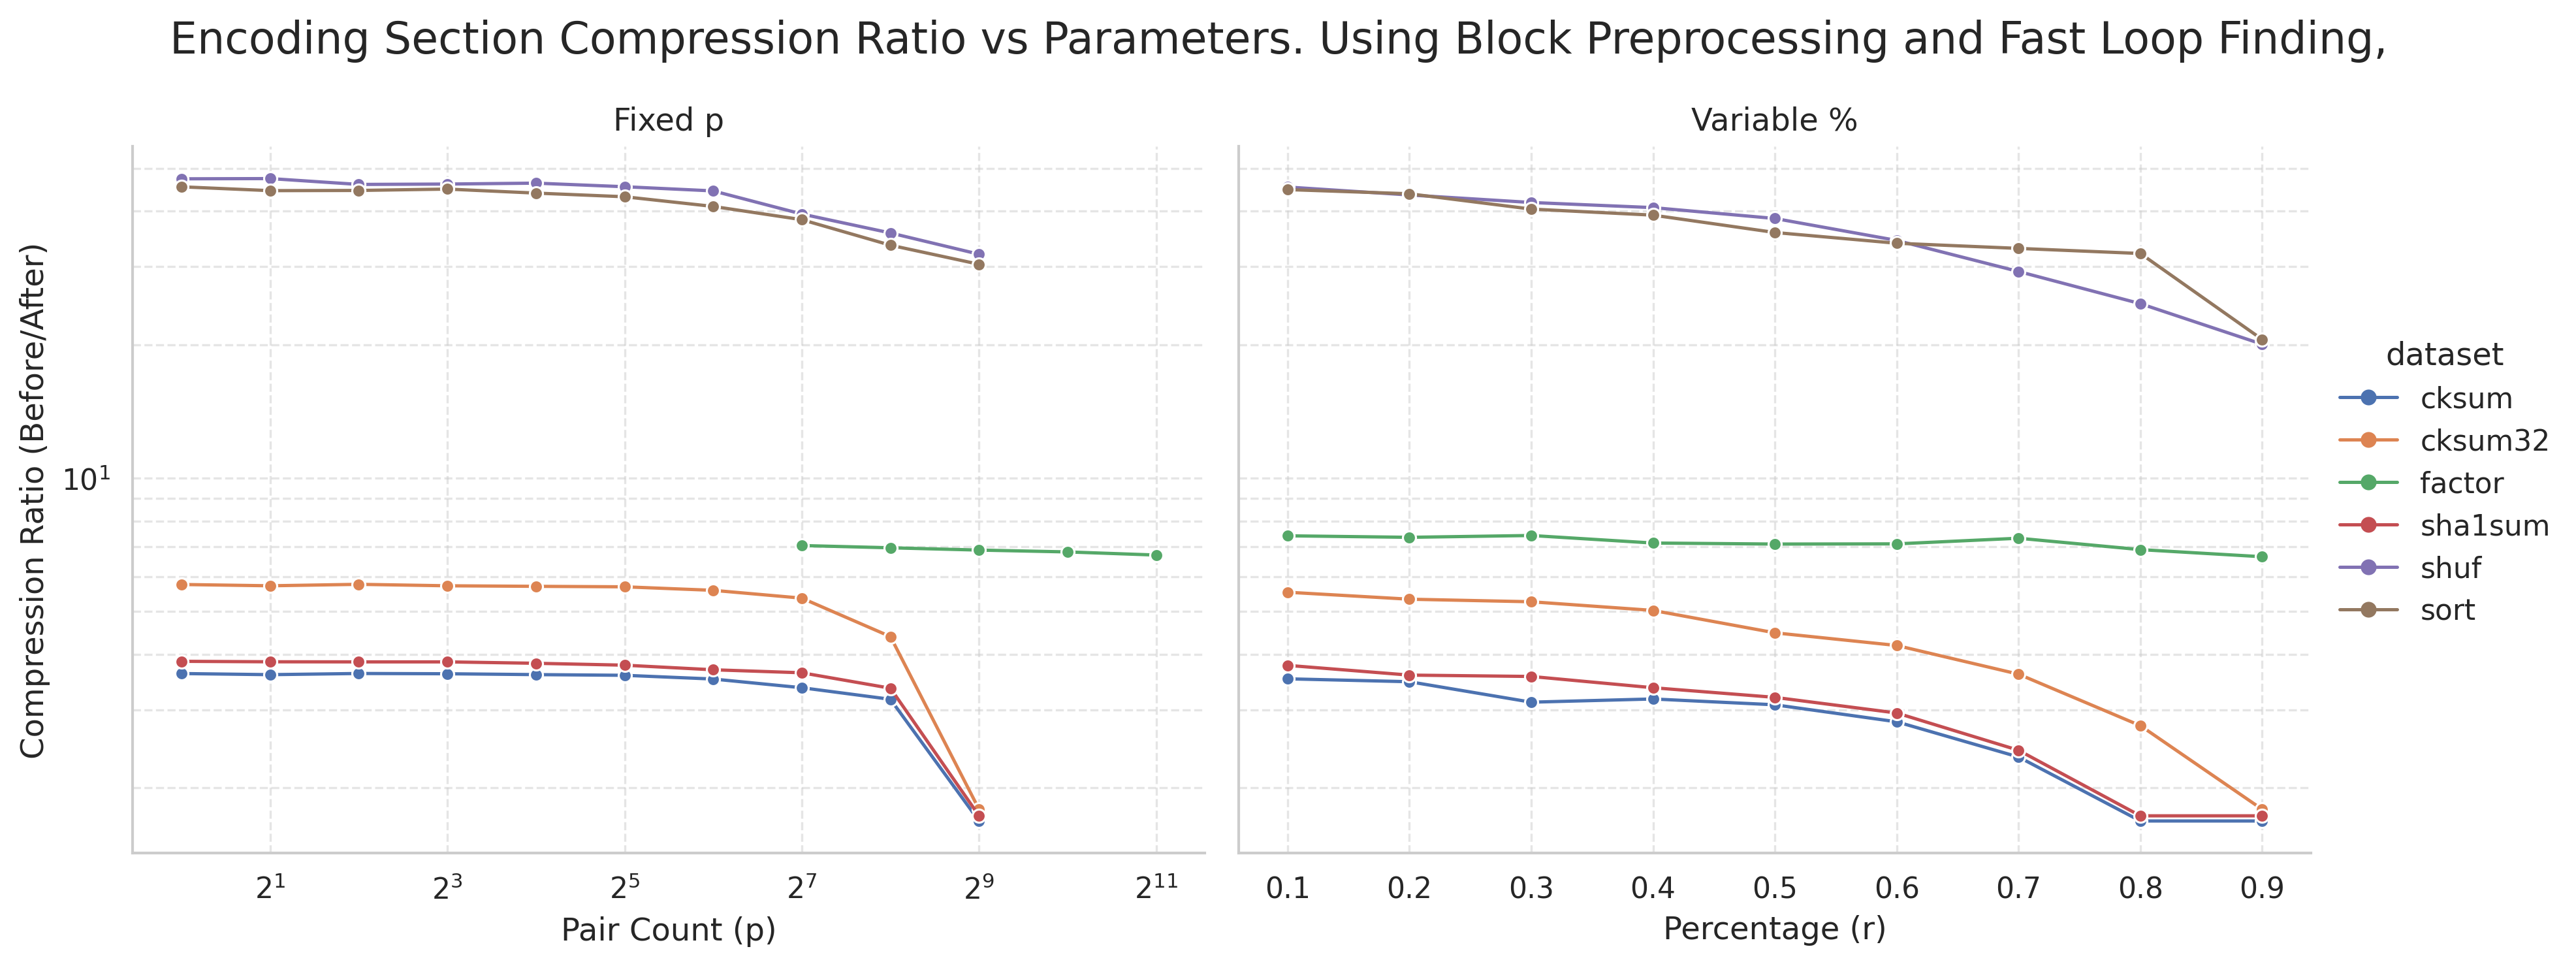
\includegraphics[width=0.8\textwidth]{graphs/encoder_compression_loop.png}
  \caption{Comparing runtime of program on different datasets, for different encoder parameters, including block 
  preprocessing and loop finding.}
  \label{eval:fig:encoder-block-loop-comp}
\end{figure}

expression size vs iteration

\begin{figure}[htbp]
  \centering
  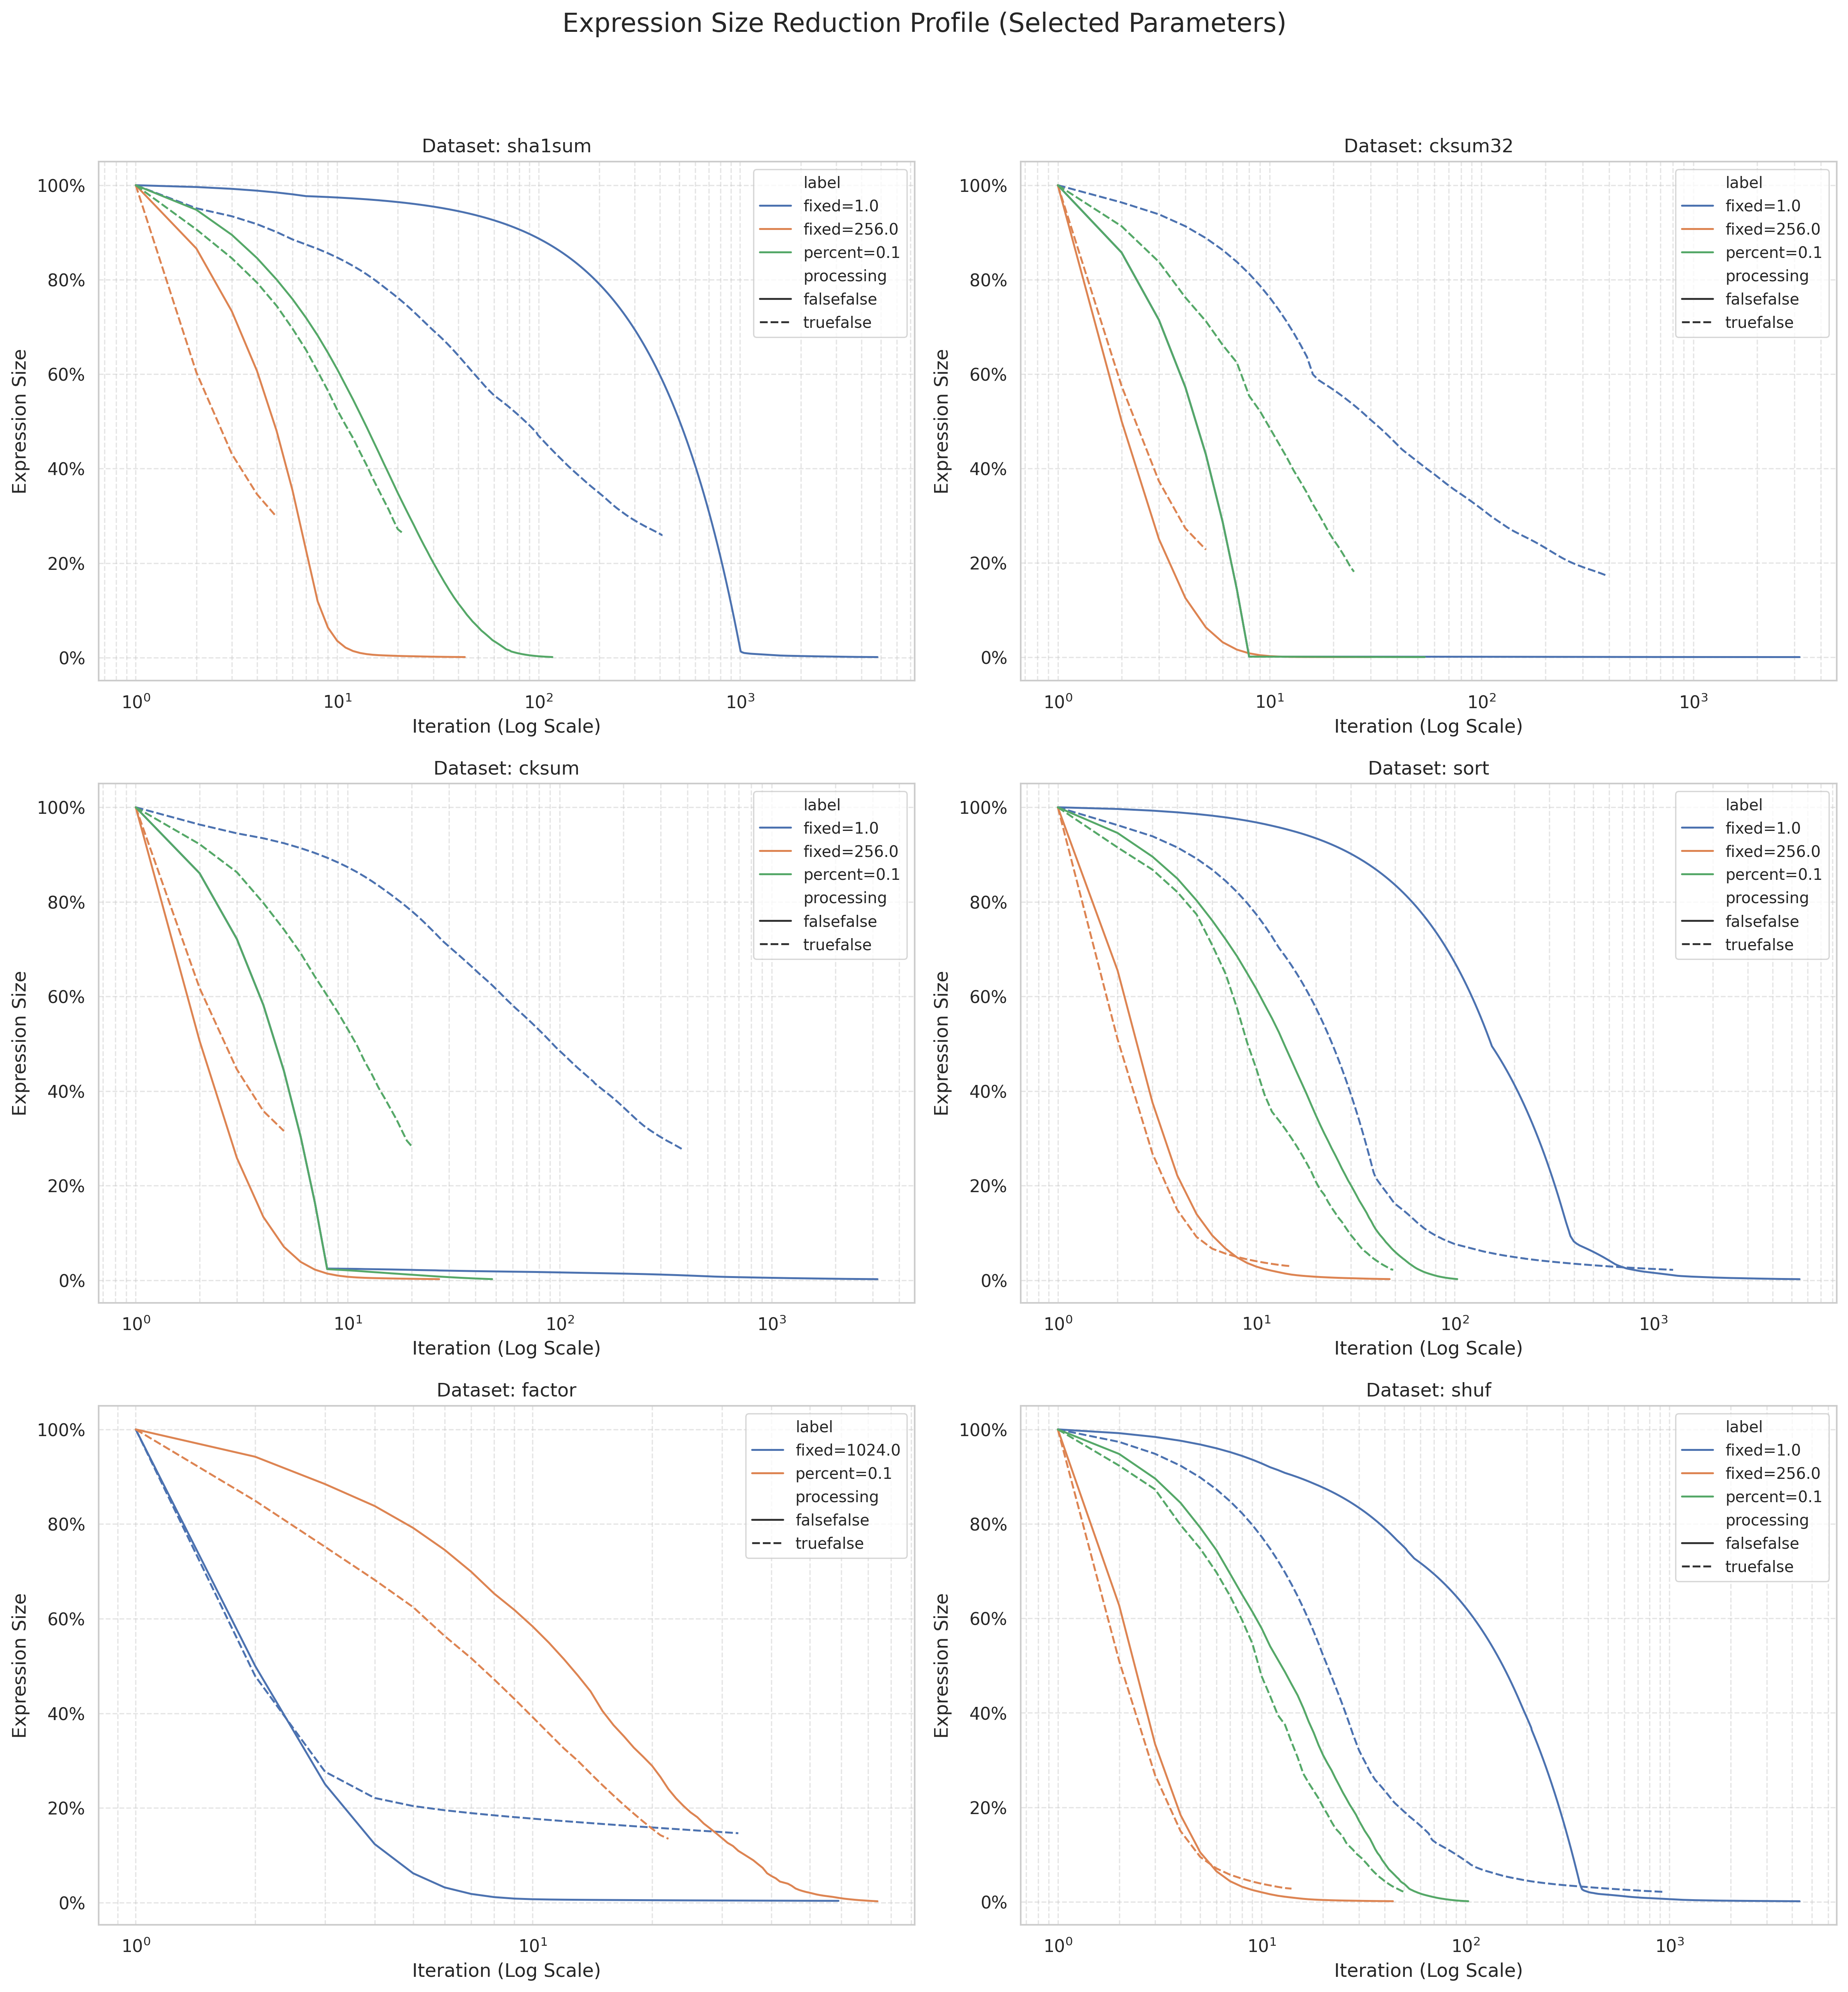
\includegraphics[width=1\textwidth]{graphs/encoder_profile.png}
  \caption{Comparing reduction behaviour of encoder on different datasets, for representative parameters.}
  \label{eval:fig:encoder-profile}
\end{figure}

Table for mults vs iterations for no processing, block processing, loop finding

\begin{table}[ht]
\begin{center}
\begin{tabular}{lcccc}
  \textbf{Dataset} & \textbf{Blocks} & \textbf{Fast Loops} & \textbf{Multiplications} & \textbf{Iterations} \\
  \midrule
  cksum \\
  cksum \\
  cksum \\
  cksum32\\
  cksum32\\
  cksum32\\
  factor\\
  factor\\
  factor\\
  sha1sum\\
  sha1sum\\
  sha1sum\\
  shuf \\
  shuf \\
  shuf \\
  sort\\
  sort\\
  sort\\
  \midrule
\end{tabular}
\end{center}
\caption{Summary of total multiplications and encoder iterations on the selected data.}
\label{tbl:single-thread-mults}
\end{table}

time tradeoff for each pipeline component

\begin{figure}[htbp]
  \centering
  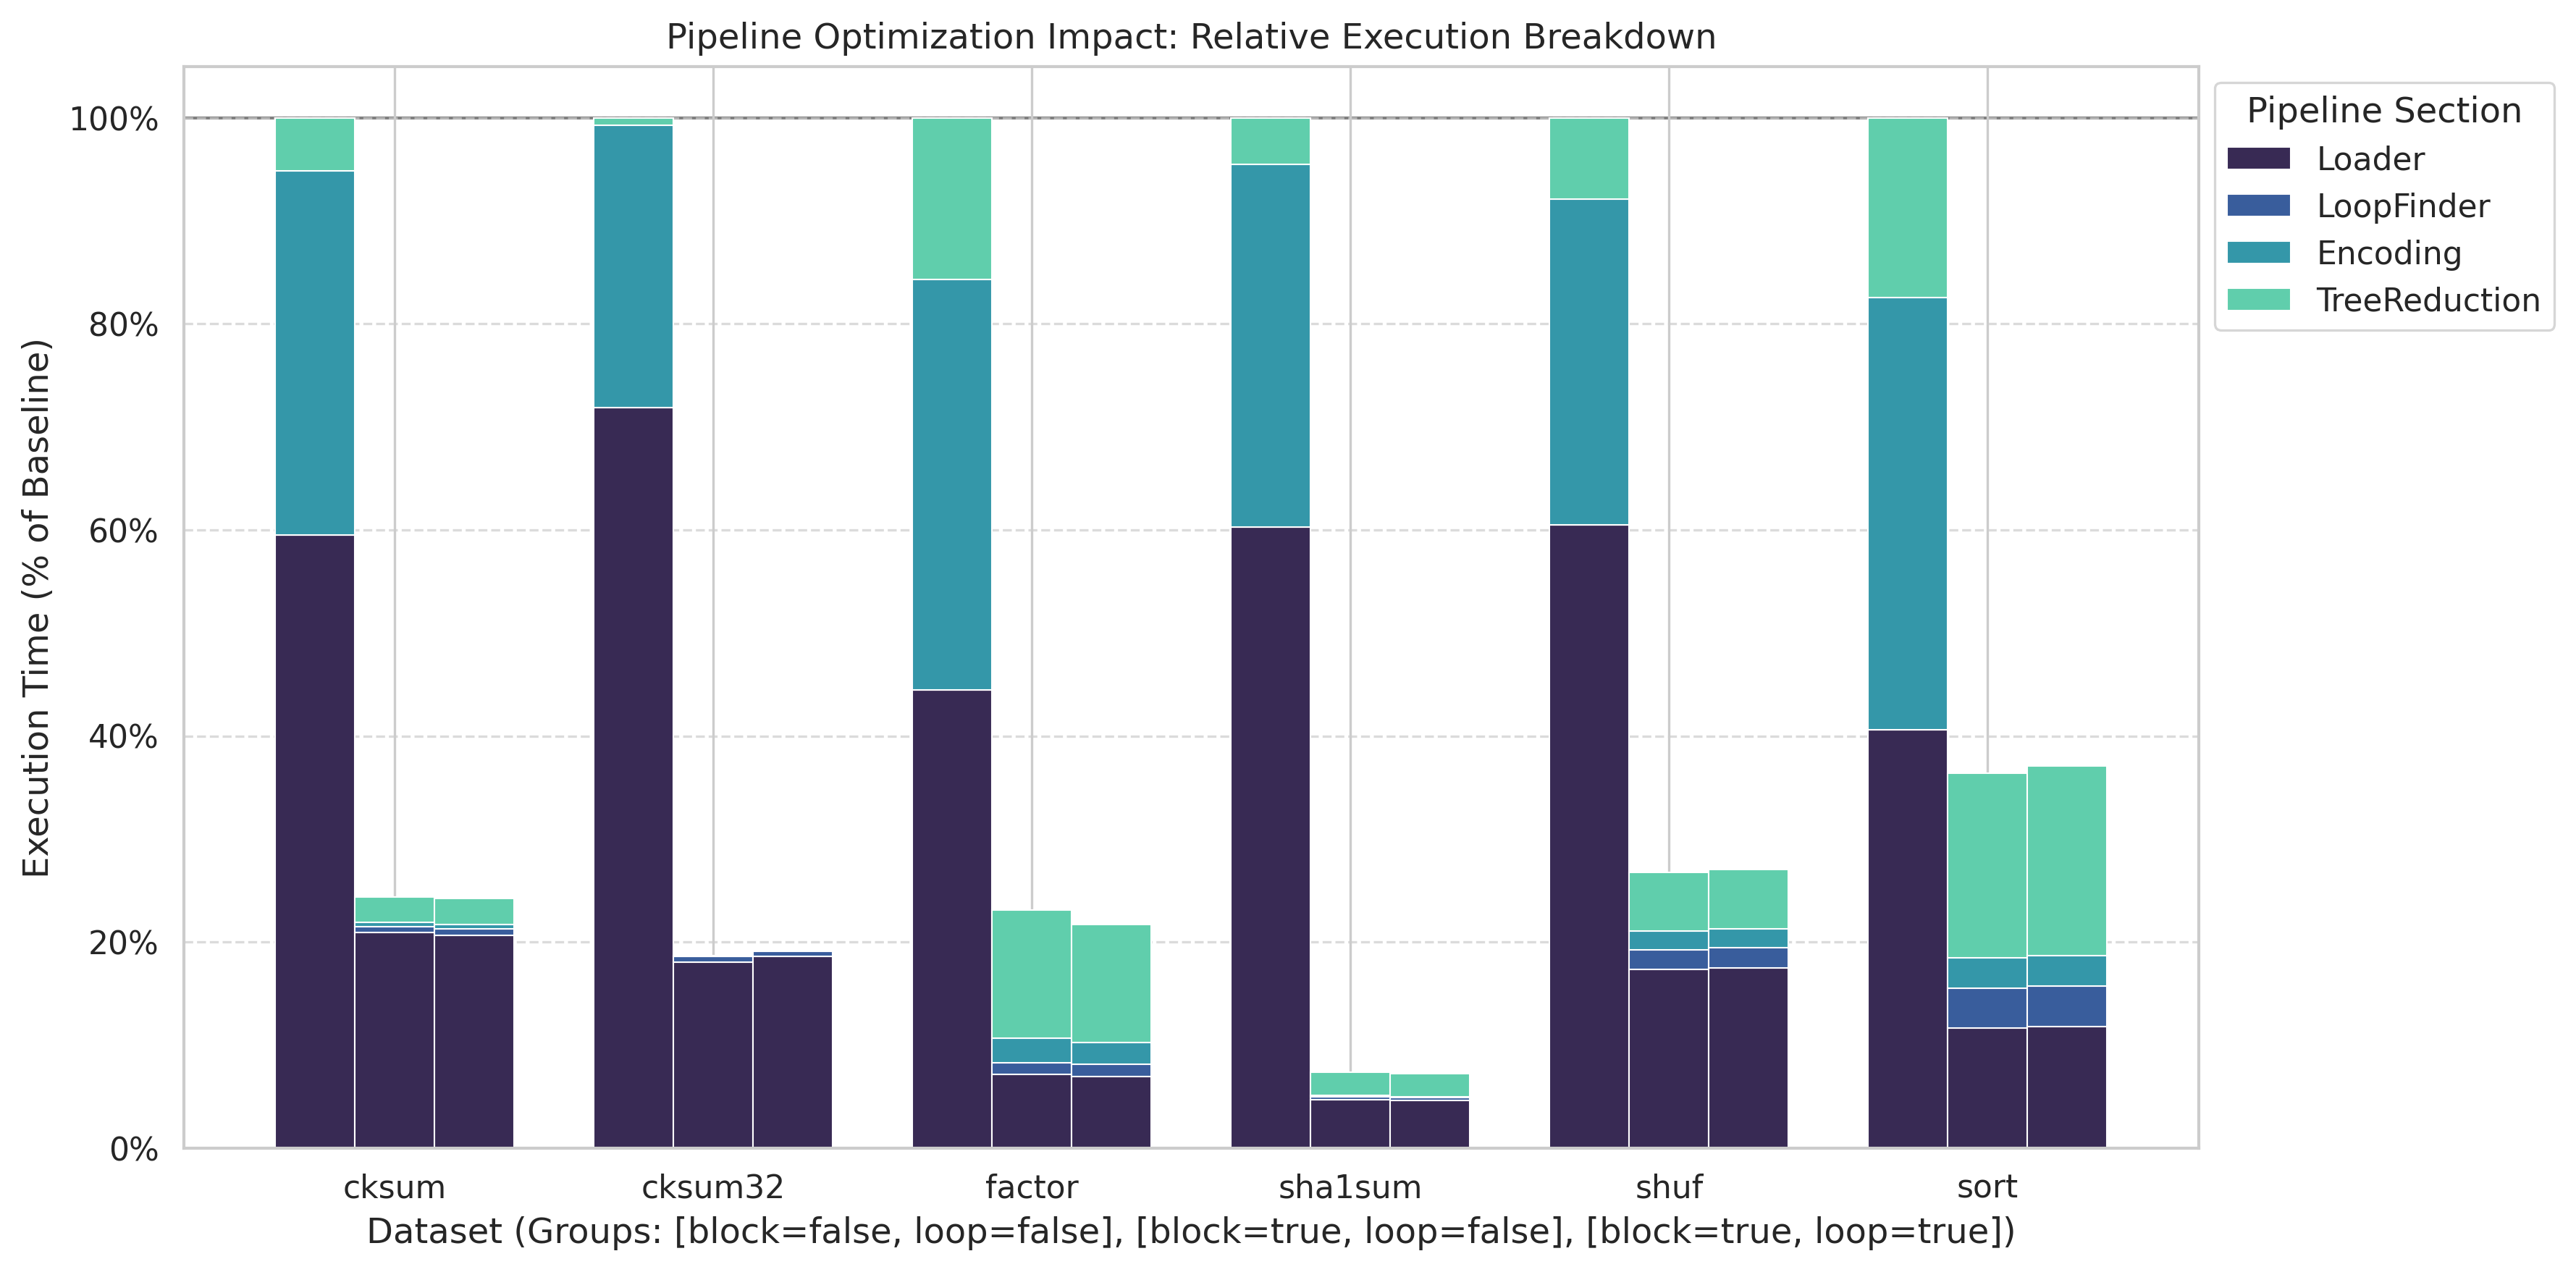
\includegraphics[width=1\textwidth]{graphs/pipeline_optimization.png}
  \caption{Comparing the speedup for block preprocessing and fast loop finding}
  \label{eval:fig:single-thread-speedup}
\end{figure}

\section{Concurrency and GPU deep dive}

encoder time performance (directly from program execution) with threads and chunks

encoder efficiency! with chunk count

multiplication performance (artificial benchmark so we can make sure multiplier doesnt starve for huge multiiplication counts) with threads

GPU timeline

\section{Memory profiling}

bar chart maximum resident set size 

line graph heap memory allocation

\section{Holistic Pipeline}
